
\medskip

\textbf{Question 1}

\medskip

$f(-1) = \left(4 \times (-1) - 1\right)\e^{-1} = (-4 - 1)\e^{-1} = -5\e^{-1} = -\dfrac{5}{\e}$.

\bigskip

\textbf{Question 2}

\medskip

$\ds\lim_{x\to +\infty} 4x - 1 = +\infty \quad$ et $\quad \ds\lim_{x\to +\infty} \e^x = +\infty \quad$, d'où :
\[\lim_{x \to +\infty} f(x) = \lim_{x \to +\infty} (4x - 1)\e^x = +\infty.\]

\bigskip

\textbf{Question 3}

\medskip

\begin{enumerate}
\item $f'(x) = \left(4x - 1\right) \times \e^x + 4 \times \e^x = \e^x \left(4x - 1 + 4\right) = \e^x (4x + 3).$

\item Résolution de $f'(x) = 0$, soit $\e^x (4x + 3) = 0$.

$\e^x > 0$, donc : $\quad 4x + 3 = 0 \quad \Longrightarrow \quad x = -\dfrac{3}{4}$.

Valeur en $x = -\dfrac{3}{4}$ :
\[f\left(-\dfrac{3}{4}\right) = \left(4 \times \left(-\dfrac{3}{4}\right) - 1\right)\e^{-\frac{3}{4}} = (-3 - 1)\e^{-\frac{3}{4}} = -4\e^{-\frac{3}{4}}.\]

\begin{center}
\begin{tikzpicture}
\tkzTabInit[lgt=2.5, espcl=3]{$x$ / 1, {$\e^x$} / 1, {$4x + 3$} / 1, {Signe de $f'(x)$} / 1, {Variations de $f$} / 2}{${-1}$, ${-\frac{3}{4}}$, ${+\infty}$}
\tkzTabLine{,+,d,+,}
\tkzTabLine{,-,0,+,}
\tkzTabLine{,-,0,+,}
\tkzTabVar{+/{$$},-/{$-4\e^{-\frac34}$},+/{$$}}{/}
\end{tikzpicture}
\end{center}

\end{enumerate}

\bigskip

\textbf{Question 4}

\medskip

$I = \ds\int_{-1}^{2} (4x - 1) \, dx = \left[2x^2 - x\right]_{-1}^{2} = \left(2 \times 4 - 2\right) - \left(2 \times 1 - (-1)\right) = (8 - 2) - (2 + 1) = 6 - 3 = 3.$

\bigskip

\textbf{Question 5}

\medskip

$\ln(576) = \ln(2^6 \times 3^2) = \ln(2^6) + \ln(3^2) = 6\ln(2) + 2\ln(3)$.

\bigskip

\textbf{Question 6}

\medskip

On applique la formule d'Al-Kashi :
\begin{align*}
AC^2 &= AB^2 + BC^2 - 2 \times AB \times BC \times \cos\, (60^\circ) \\
&= 10^2 + 4^2 - 2 \times 10 \times 4 \times \dfrac{1}{2} \\
&= 100 + 16 - 40 \\
&= 76.
\end{align*}
Soit : $AC = \sqrt{76} = 2\sqrt{19} \approx 8,7$ au dixième près.

\bigskip


